\documentclass[lettersize,journal]{IEEEtran}
\usepackage{colortbl}
\usepackage{amsmath,amssymb}
\usepackage{tikz}
\usetikzlibrary{arrows,fit,positioning,shapes,patterns}
\usepackage{pgfplots}
\pgfplotsset{width=8cm,compat=1.9}

\begin{document}

    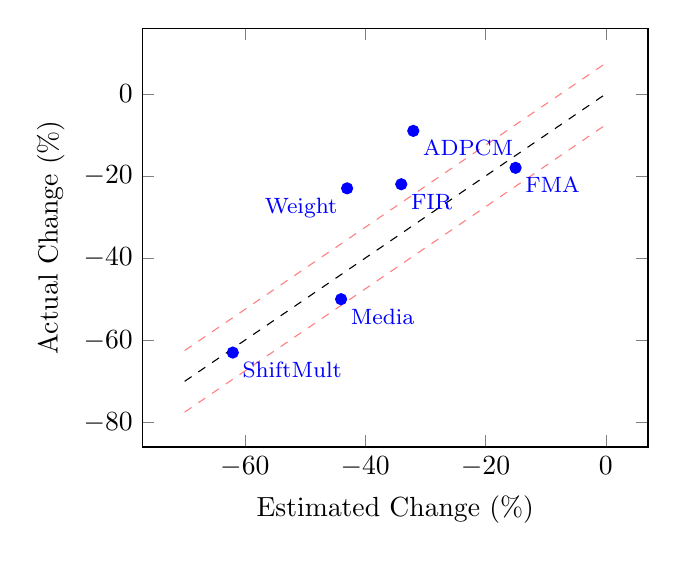
\begin{tikzpicture}

\begin{axis}[xlabel=Estimated Change (\%),ylabel= Actual Change (\%)]
    \addplot[
    color=black,
    dashed
    ]
    coordinates {
    (-70,-70)(0,0)
    };

    \addplot[
    color=red!50,
    dashed
    ]
    coordinates {
    (-70,-77.5)(0,-7.5)
    };

    \addplot[
    color=red!50,
    dashed
    ]
    coordinates {
    (-70,-62.5)(0,7.5)
    };

    \addplot[%
    scatter/classes={a={blue}, b={red}},
        scatter, mark=*, only marks, 
        scatter src=explicit symbolic,
        nodes near coords*={\Label},
         every node near coord/.append style={anchor=north west, font=\footnotesize},
        visualization depends on={value \thisrow{label} \as \Label},
        color=blue
    ] table [meta=class] {
x y class label
-34 -22 a FIR
-44 -50 a Media
-32 -09 a ADPCM
-15 -18 a FMA
-62 -63 a ShiftMult
% -43 -23 a Weight
    };

\addplot[mark=*, color=blue, nodes near coords={\footnotesize Weight}, every node near coord/.style = {anchor=north east, align=center, color=blue}, only marks]
 coordinates {(-43, -23)};

\end{axis}
\end{tikzpicture}

\end{document}